\documentclass{article}

\usepackage{lipsum}
\usepackage[nocheck]{fancyhdr}
\usepackage{graphicx}



\pagestyle{fancy}
\rhead{Management Software for Informal Businesses}
\rfoot{St. Paul's University}


\begin{document}
\renewcommand{\familydefault}{\sfdefault}
\renewcommand{\baselinestretch}{1.5}
\setlength{\parskip}{0.5em}
\setlength{\parindent}{0pt}
\setlength{\textwidth}{6.5in}
\setlength{\textheight}{9.5in}
\setlength{\topmargin}{-0.5in}

\thispagestyle{empty}
\begin{center}
	{\bfseries\huge
		St. Paul's University \\
		BAR 4102A \\
		IT Business Research Project \\
		Charles Kamiri  \\
		BOBITNRB200621 \\ [60pt]
	}

\emph{Management Software for Informal Businesses}
\end{center}
\newpage


% Table of Contents
\thispagestyle{empty}
\renewcommand{\contentsname}{Table of Contents}
\tableofcontents
\newpage


% Introduction
\section{Introduction}
\subsection{Background}
\paragraph{}
Informal businesses, also known as micro, small, and medium enterprises (MSMEs), are a critical component of the global economy. These businesses provide employment opportunities and contribute to economic growth in many developing countries.

\subsection{Problem Statement}
\paragraph*{}
HoIver, most informal businesses face several challenges, such as limited access to financial resources, lack of business skills, and poor record-keeping practices. These challenges hinder the growth and sustainability of these businesses, limiting their potential to contribute to the economy.

\subsection{Objectives}
\paragraph*{}
To address these challenges, I propose the development of a management software specifically designed for informal businesses. The software aims to provide a simple, affordable, and accessible solution to help these businesses manage their operations effectively. The software will offer features such as inventory management, sales tracking, financial management, and customer relationship management. With these features, informal businesses will be able to keep accurate records, make informed decisions, and improve their profitability.

\subsection{Justification}
\paragraph*{}
Our proposed management software is designed to be user-friendly, affordable, and accessible to all types of informal businesses, regardless of their level of technical expertise. I believe that this software can have a significant impact on the growth and sustainability of informal businesses, leading to more significant contributions to the economy.

\subsection{Limitations}
\paragraph*{}
Limited access to technology: Many informal businesses may not have access to the necessary technology, such as computers or smartphones, to use the management software effectively. This could limit the potential reach and impact of the software.

\paragraph*{}
Limited data availability: Informal businesses may not have access to the same level of data as formal businesses, making it more difficult to develop accurate and reliable management software. This could result in incomplete or inaccurate information being used to make business decisions.

\paragraph*{}
Limited financial resources: Many informal businesses operate on very limited budgets, which may make it difficult for them to afford the cost of the software or the hardware required to use it.

\paragraph*{}
Limited technical expertise: Informal business owners may not have the technical expertise required to use the management software effectively, which could limit its usefulness and adoption.

\paragraph*{}
Resistance to change: Some informal businesses may be resistant to adopting new technology or changing their existing business practices, which could limit the adoption and effectiveness of the management software.

\paragraph*{}
Limited scalability: If the management software is not designed to be scalable, it may not be able to handle the growing needs of businesses as they expand, potentially limiting its usefulness over time.

\paragraph*{}
Lack of integration with existing systems: If the management software is not designed to integrate with existing systems or software used by informal businesses, it may not be used effectively or may require additional work to use alongside existing tools.
\newpage


% Literature Review
\section{Literature Review}
\paragraph*{}
Management software for informal businesses has gained attention in recent years due to its potential to improve business performance. Several studies have explored the use of management software by informal businesses, identifying its benefits and challenges.

\paragraph*{}
A study by Akter and colleagues (2019) examined the adoption of management software among informal businesses in Bangladesh. The study found that the use of software significantly improved business performance, including sales growth and profitability. HoIver, the study also identified several challenges, including the lack of technical expertise and infrastructure.

\paragraph*{}
Similarly, a study by Fuchs and colleagues (2021) examined the impact of a mobile-based management system on microenterprises in Tanzania. The study found that the system improved businesses' ability to manage inventory and finances, leading to increased sales and profitability. The study also highlighted the importance of user-friendly software and training to overcome barriers to adoption.

\paragraph*{}
Another study by Yumusak and colleagues (2021) investigated the factors influencing the adoption of management software by informal businesses in Turkey. The study found that businesses Ire more likely to adopt software if they perceived it to be useful, easy to use, and compatible with their existing systems. The study also highlighted the importance of social networks in promoting software adoption among informal businesses.

\paragraph*{}
The research revieId in this literature review suggests that management software can significantly improve the performance of informal businesses. HoIver, the adoption of software by informal businesses faces several challenges, including technical expertise, infrastructure, user-friendliness, and compatibility with existing systems. Addressing these challenges through training and social networks can help to promote the adoption of management software by informal businesses.


\newpage

% Methodology
\section{Methodology}
%\lipsum[1-2]
\subsection{Needs Assessment}
\paragraph*{}
The first step in the methodology will be to conduct a needs assessment to identify the specific needs and requirements of the target audience. This will involve conducting interviews with informal business owners and managers to understand their current management practices and the challenges they face. The needs assessment will also involve reviewing existing literature and research on the subject to identify best practices and trends.

\subsection{Software Design}
\paragraph*{}
The second step will be to design the software based on the needs assessment findings. The software will be designed to be user-friendly, customizable, and scalable. The design will be informed by the latest software development technologies and practices.

\subsection{Software Development}
\paragraph*{}
The third step will be to develop the software based on the design specifications. The software will be developed using an agile development methodology, which involves iterative development, continuous testing, and feedback from stakeholders. The software will be developed using open-source technologies and will be customizable to meet the specific needs of each business.

\subsection{Testing and Validation}
\paragraph*{}
The fourth step will be to test the software to ensure that it meets the requirements and specifications. This will involve conducting user acceptance testing (UAT) with informal business owners and managers to validate the software's functionality and ease of use. The software will also be tested for security, reliability, and scalability.

\subsection{Deployment and Training}
\paragraph*{}
The fifth step will be to deploy the software to the target audience and provide training and support. The deployment process will involve installing the software on each business's computers and configuring the software to meet their specific needs. Training will be provided to ensure that users are familiar with the software's features and capabilities. Support will be provided to address any issues or concerns that arise during the deployment and training process.

\subsection{Monitoring and Evaluation}
\paragraph*{}
The final step will be to monitor and evaluate the software's effectiveness in improving the productivity, efficiency, and profitability of informal businesses. This will involve collecting data on key performance indicators (KPIs) such as sales, expenses, and profits, and analyzing the data to assess the impact of the software. Feedback from users will also be solicited to identify areas for improvement and future development.

Overall, this methodology will ensure that the software system meets the needs and requirements of informal businesses and contributes to their growth and success.
\newpage


% Implantation
\section{Implantation}

\subsection{Project Timeline}

The following table outlines the project timeline, milestones, and deadlines for different phases of the project:

\begin{table}[htbp]
\centering
\caption{Project Timeline}
\begin{tabular}{|c|c|}
\hline
\textbf{Phase} & \textbf{Timeline} \\
\hline
Requirements gathering & Week 1 \\
Design & Week 2 - 4 \\
Development & Months 2 -3 \\
Testing & Months 4 \\
Deployment & Month 4 \\
Maintenance & Ongoing \\
\hline
\end{tabular}%
\label{tab:timeline}%
\end{table}%

\subsection{Project Budget}

The following table describes the resources needed to carry out the project, as well as the estimated costs associated with each resource:

\begin{table}[htbp]
\centering
\caption{Project Budget}
\begin{tabular}{|c|c|}
\hline
\textbf{Resource} & \textbf{Estimated Cost} \\
\hline
Personnel (developers, project manager) & Ksh. 50,000 \\
Equipment (computers, software licenses) & Ksh. 25,000 \\
Materials (office supplies, documentation) & Ksh. 1, 000 \\
\hline
\textbf{Total} & \textbf{Ksh. 76,000} \\
\hline
\end{tabular}%
\label{tab:budget}%
\end{table}%

\subsection{Risk Management}

The following table describes the potential risks associated with the project and how these risks will be managed or mitigated:

\begin{table}[htbp]
\centering
\caption{Risk Management}
\begin{tabular}{|c|c|}
\hline
\textbf{Risk} & \textbf{Mitigation} \\
\hline
Delays in development & Regular progress reports and milestone tracking \\
Technical difficulties & Experienced development team and backup resources \\
Inadequate testing & Thorough testing plan and user feedback \\
Lack of user adoption & User-centered design and training \\
\hline
\end{tabular}%
\label{tab:risk}%
\end{table}%

\subsection{Evaluation and Monitoring}

The following figure outlines how the project's progress will be monitored, evaluated, and reported, as Ill as how the project's success will be measured against its goals and objectives:

\begin{figure}[htbp]
\centering
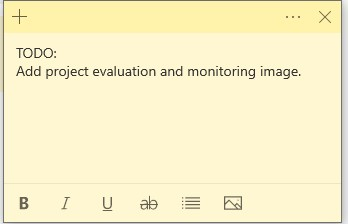
\includegraphics[width=0.8\textwidth]{evaluation.jpg}
\caption{Project Evaluation and Monitoring}
\label{fig:evaluation}
\end{figure}
\newpage


% Testing
\section{Testing}
\label{sec:testing}

The testing approach for the management software project will focus on ensuring that the software is functional, reliable, and performs Ill. I will use a combination of automated and manual testing techniques to test the software.

\subsection{Testing Approach}
I will use the Agile testing methodology to ensure that testing is integrated into the development process. This will include continuous testing, where I will run automated tests as part of the continuous integration and deployment process.

For manual testing, I will have a team of testers who will test the software at various stages of development, including integration testing and user acceptance testing. The testing phase will run closely with the development phase to ensure that defects are identified and resolved in a timely manner.

\subsection{Testing Scope}
The testing scope for our project will cover the following areas:

\begin{itemize}
\item Functional testing: I will test the various features of the management software to ensure that they work as expected, including user registration, inventory management, and financial reporting.
\item Integration testing: I will test the integration of the frontend (React) and backend (Java Spring Boot) components to ensure that they work seamlessly together.
\item Performance testing: I will test the performance of the software under various loads to ensure that it can handle high traffic and usage.
\item Security testing: I will test the security of the software to ensure that it is protected against common security threats, such as SQL injection and cross-site scripting.
\end{itemize}

\subsection{Testing Resources}
To conduct the testing activities, I will need the following resources:

\begin{itemize}
\item Hardware: I will require a dedicated testing environment with suitable hardware resources to simulate real-world usage scenarios.
\item Software: I will use a combination of open source and commercial testing tools, including JUnit, Selenium, and Apache JMeter.
\end{itemize}

\subsection{Testing Plan}
The testing plan will include the following activities:

\begin{itemize}
\item Test case development: I will develop a set of test cases that cover the various features and functionalities of the software.
\item Test execution: I will execute the test cases to ensure that the software meets the requirements and specifications.
\item Test reporting: I will document the results of the testing activities and report any defects or issues to the development team for resolution.
\item Retesting: I will retest any defects or issues that are resolved in development to ensure that they have been properly fixed.
\end{itemize}

\subsection{Risk Assessment}
The following potential risks have been identified and will be mitigated as follows:

\begin{itemize}
\item Inadequate testing coverage: I will mitigate this risk by developing a comprehensive set of test cases that cover all aspects of the software.
\item Inconsistent testing: I will mitigate this risk by using a combination of automated and manual testing techniques and by having a dedicated testing team.
\item Testing delays: I will mitigate this risk by incorporating testing into the development process and by using automated testing wherever possible to minimize delays.
\end{itemize}
\newpage


% References
\section{References}
\renewcommand{\refname}{}
\begin{thebibliography}{10}
	\bibliographystyle{apalike}
	% Add references here
	\bibitem{ref1}
	Akter, S., Islam, S., \& Ahsan, M. (2019). Adoption of management software among microenterprises in Bangladesh: An empirical study. Information Development, 35(2), 265-280.

	\bibitem{ref2}
	Fuchs, C., Huesing, T., \& Schäfer, M. (2021). Mobile-based management systems for informal businesses in Tanzania: Effects on business performance and adoption barriers. Journal of Business Research, 129, 496-507.

	\bibitem{ref3}
	Yumusak, I. G., Coskun, Y., \& Ozkan-Ozen, Y. D. (2021). Factors influencing adoption of management software among small businesses: The case of Turkey. Journal of Enterprise Information Management, 34(1), 27-45.

\end{thebibliography}
\end{document}